\subsubsection*{\underline{\textsc{\Large Wraith}}}
\noindent\emph{Medium undead, neutral evil}

\noindent\rule{0.5\textwidth}{0.5pt}

\noindent\textbf{Armor Class}: 13

\noindent\textbf{Hit Points}: 67 (9d8 + 27)

\noindent\textbf{Speed}: 0 ft., fly 60 ft. (hover)

\noindent\rule{0.5\textwidth}{0.5pt}
\begin{table}[H]
	\begin{tabular}{cccccc}
		\textbf{STR} & \textbf{DEX} & \textbf{CON} & \textbf{INT} & \textbf{WIS} & \textbf{CHA} \\
		6 (-2) & 16 (+3) & 16 (+3) & 12 (+1) & 14 (+2) & 15 (+2) \\
	\end{tabular}
\end{table}
\noindent\rule{0.5\textwidth}{0.5pt}

\noindent\textbf{Saving Throws}: Wis +0

\noindent\textbf{Damage Resistances}:  acid, cold, fire, lightning, thunder; bludgeoning, piercing, and slashing from nonmagical attacks that aren't silvered

\noindent\textbf{Damage Immunities}: necrotic, poison

\noindent\textbf{Condition Immunities}: charmed, exhaustion, grappled, paralyzed, petrified, poisoned, prone, restrained

\noindent\textbf{Senses}: darkvision 60 ft., passive Perception 12

\noindent\textbf{Languages}: the languages it knew in life

\noindent\textbf{Challenge}: 5 (1800 XP)

\noindent\rule{0.5\textwidth}{0.5pt}

\noindent\textbf{Incorporeal Movement}: The wraith can move through other creatures and objects as if they were difficult terrain. It takes 5 (1d10) force damage if it ends its turn inside an object.

\noindent\textbf{Sunlight Sensitivity}: While in sunlight, the wraith has disadvantage on attack rolls, as well as on Wisdom (Perception) checks that rely on sight.

\noindent\rule{0.5\textwidth}{0.5pt}

\noindent\textbf{ACTIONS}

\noindent\textbf{Life Drain}:  Melee Weapon Attack: +6 to hit, reach 5 ft., one creature. Hit: 21 (4d8 + 3) necrotic damage. The target must succeed on a DC 14 Constitution saving throw or its hit point maximum is reduced by an amount equal to the damage taken. This reduction lasts until the target finishes a long rest. The target dies if this effect reduces its hit point maximum to 0.

\noindent\textbf{Create Specter}:  The wraith targets a humanoid within 10 feet of it that has been dead for no longer than 1 minute and died violently. The target's spirit rises as a specter in the space of its corpse or in the nearest unoccupied space. The specter is under the wraith's control. The wraith can have no more than seven specters under its control at one time.

\begin{center}
	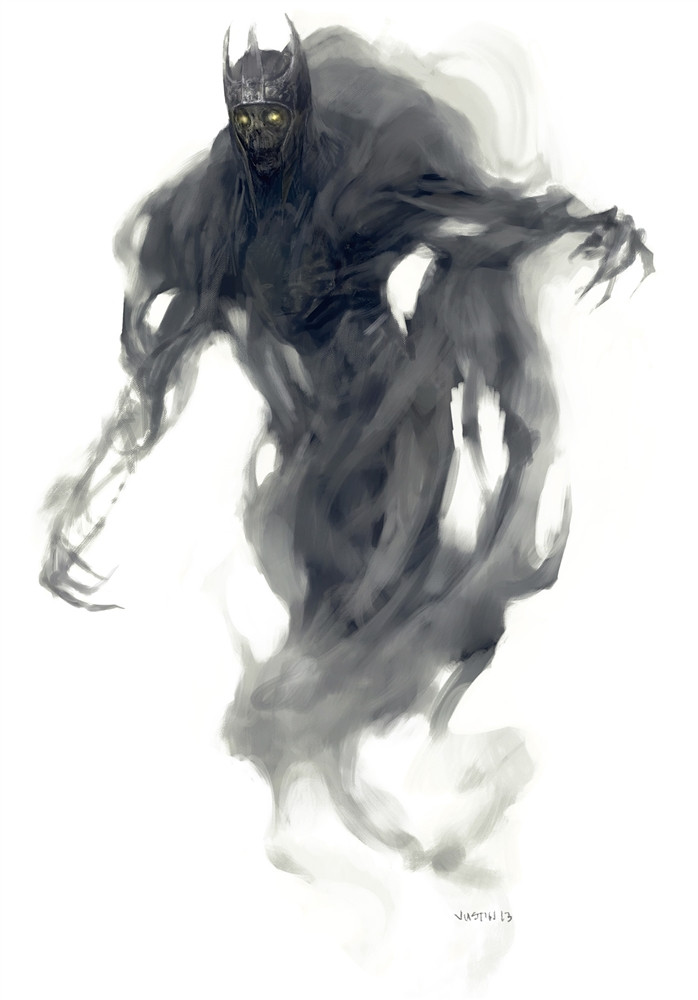
\includegraphics[width = 0.3\textwidth]{wraith}
	
	\emph{Wraith}
\end{center}